\chapter{Materials \& Methods}

% 학위 논문의 결과를 도출하는 데에 사용한 실험 재료와 방법을 타인이 반복 실험 시 동일한 결과를 얻을 수 있을 정도로 자세히 기술한다. 방법에 따라 다음과 같이 부제를 넣어 기술한다.f

% 예)
% 2.1 식물 재료 및 생장 조건
% 2.2 뿌리 관속 조직 관찰
% 2.3 유전자 발현 분석

\section{Space Optimization}

\subsection{Diff-index Compression}

As is described in chapter 2, the diff-index created in the k-mer extraction step will store multiple \texttt{USHRT\_MAX} as long as the difference is larger than \texttt{USHRT\_MAX}. This will make any k-mer difference larger than $4 \times \mathtt{USHRT\_MAX} = 262140$ require a larger space to store than the original \texttt{unsigned long} representation. This situation is not uncommon especially when $k$ is large.
Also, in the prototypical implementation, the ID of sthe source sequence will also be stored multiple times in the ID table. This redundancy is both unnecessary and troublesome. It will increase the size of \texttt{Petasearch} data structures even more than the repeated \texttt{USHRT\_MAX} since the IDs are stored as \texttt{unsigned long} (64-bit integers).
\autoref{fig:k11_space} showed the space consumption of the diff-index created in the k-mer extraction step when $k = 11$. Without optimization, the diff-index (k-mer table) and its corresponding ID table will take up 17 GB of space for a merely 1GB-sized database.

To optimize the size of the diff-index, we devised the bit-squeezing technique to compress the difference between two adjacent k-mers:
For any 64-bit k-mer difference, we continuously fetch 15 bits into a write buffer starting from the least significant bits. We stop the retrieval until we encounter a zero chunk (15 bits of zeros).
To enable the correct decoding of the diff-index during the next phase, the sign bit of the last element in th write is set to \texttt{1} to indicate the end of encoding. Afterwards, we write all the elements in the write buffer to the diff-index. An example encoding process for differecne of value $2039432531946$ is shown in \autoref{fig:bit_squeeze_technique}. For ID table, the optimization is simple: we store the ID of the source sequence only once instead of repeatedly.
Using the bit-squeezing method, it is possible to obtain a maximum of five chunks, making the final space consumption larger than the size of a \texttt{unsigned long} integer. However, such situation only happens when the difference is larger than $\texttt{1UL << 59} = 576460752303423488$, which is extremely rare.

While decoding the compressed diff-index in the process of double-index search, we will reverse the bit-squeezing process through repeatedly retrieving 15 bits from the diff-index table until we encounter the chunk with the sign bit set to \texttt{1}. The decoded difference value will be add to the current k-mer. Moreover, since we do not store redundant IDs, the ID pointer will not be incremented until the end of k-mer decoding. \cref{algorithm:decode_kmer} showed the simplified pseudocode for k-mer decoding.

\begin{algorithm}[htbp]
  \begin{algorithmic}
    \Procedure{DecodeKmer}{$currentKmer$, $currentTargetKmerPtr$, $currentTargetIDPtr$}

    \State $currentDiffIndex \gets 0$\;
    % \State $X \gets x$
    % \State$ $N \gets n$
    \While{$*currentTargetKmerPtr > 0 $}\Comment{This means the sign bit is not 1. }
    \State $currentDiffIndex \gets\ \textsc{Get15Bits}(*currTargetKmerPtr)$
    \State $currentDiffIndex \gets currentDiffIndex \texttt{ << } 15$
    \State $\textsc{Next}(currTargetKmerPtr)$
    \EndWhile
    \State $currentDiffIndex \gets\ \textsc{Get15Bits}(*currTargetKmerPtr)$
    \State $currentKmer \gets currentKmer + currentDiffIndex$
    \State $\textsc{Next}(currTargetKmerPtr)$
    \State $currentTargetIDPtr \gets\ \textsc{Next}(currentTargetIDPtr)$
    \Return $currentKmer$
    \EndProcedure
    \caption{ Pseudocode for the k-mer decoding process} \label{algorithm:decode_kmer}
  \end{algorithmic}
\end{algorithm}


\begin{figpage}
  \begin{figure}
    \centering
    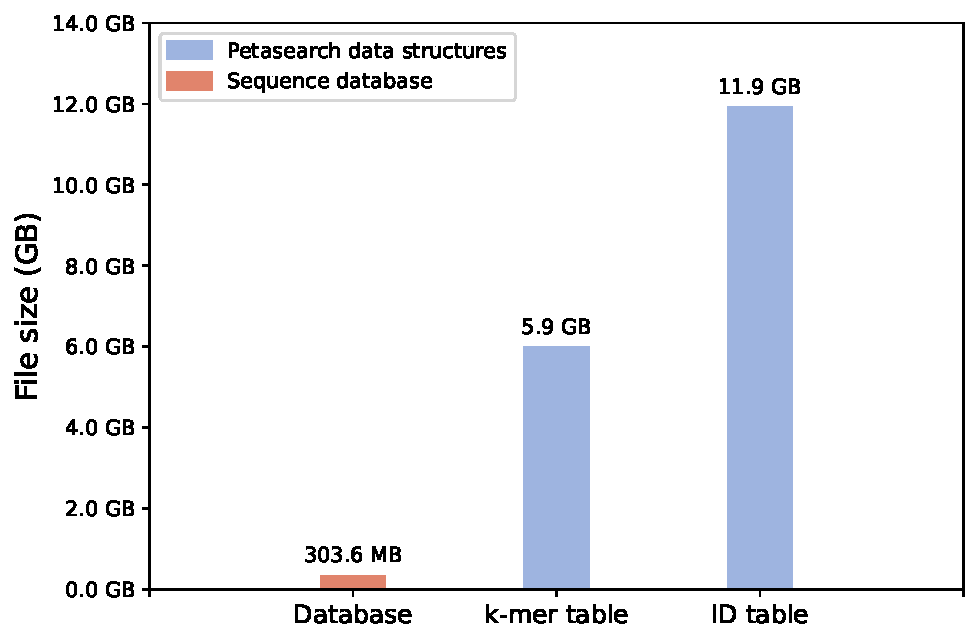
\includegraphics[width=.8\textwidth]{images/k11_space_consumption.pdf}
    \captionof{figure}{Visualizaiton of k-mer table and ID table sizes when $k = 11$. The database is the \texttt{UniProtKB/Swiss-Prot} database obtained through \texttt{mmseqs databases UniProtKB/Swiss-Prot swissprot tmp} command. Without optimization, the sizes of \texttt{petasearch} data structures are 6.46 times and 12.92 times larger than the sequence database.}
    \label{fig:k11_space}
  \end{figure}
  \begin{figure}
    \centering
    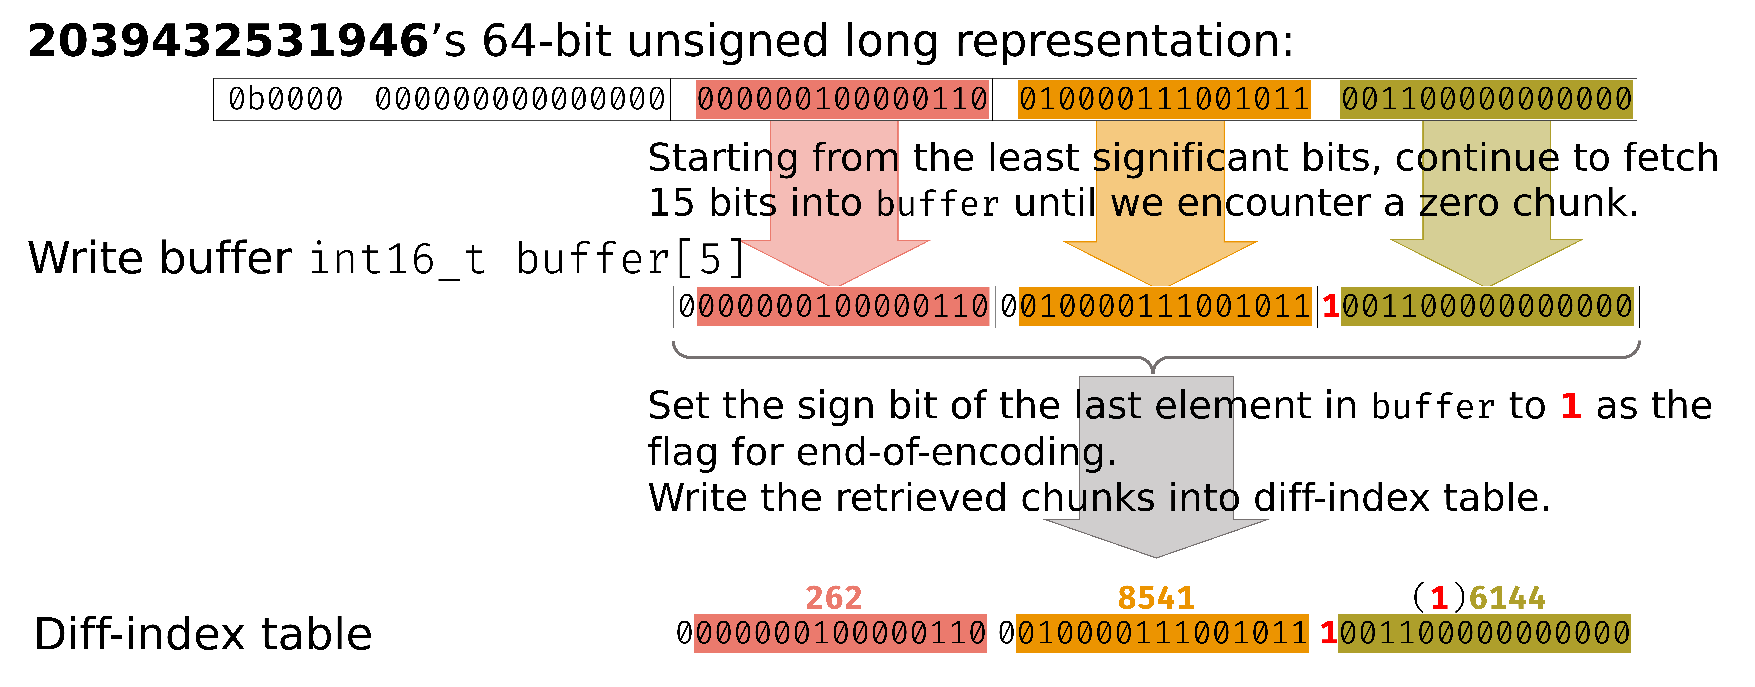
\includegraphics[width=\textwidth]{images/bit_squeezing_technique.pdf}
    \captionof{figure}{The example decoding process of difference index $2039432531946$. We first retrieve 15-bit chunks starting from the least significant bits and store them into a write buffer in the reverse order until we encounter a zero chunk. For $2039432531946$, its highest non-zero bit is $39$, which means that we need three 16-bit \texttt{short} to store it.}
    \label{fig:bit_squeeze_technique}
  \end{figure}
\end{figpage}

\section{Speed Optimization}

\subsection{}

\section{Sensitivity Improvement}
